%Title of section
\section{容器负载预测模型}

\subsection{模型结构}

\begin{frame}
\frametitle{模型结构}
\framesubtitle{引言}
\begin{itemize}
    \item 单值预测模型:ARIMA、Kalman滤波、神经网络、……
    \begin{itemize}
        \item \textbf{误差敏感} $\Rightarrow$ \textbf{决策失效}
        \item \textbf{鲁棒性差} $\Rightarrow$ \textbf{决策过度}
    \end{itemize}
    \item 区间预测模型:贝叶斯、回归模型、随机森林、……
    \begin{itemize}
        \item \textbf{预测区间} $\Rightarrow$ \textbf{目标不确定性(包含误差)}
        \item \textbf{区间置信度} $\Rightarrow$ \textbf{适合决策}
        \item \alert{\textbf{先预测再扩展为区间} $\Rightarrow$ \textbf{先验假设}}
        \item \alert{\textbf{相同分布假设} $\nRightarrow$ \textbf{适应不同类型负载}}
    \end{itemize}
    \item 基于趋势感知的区间预测模型:SAC-GPSO-SVM
    \begin{itemize}
        \item \textbf{趋势感知} $\Rightarrow$ \textbf{平稳型、趋势型和周期型负载}
        \item \textbf{区间构造} $\Rightarrow$ \textbf{针对不同负载类型}
        \item \textbf{区间预测} $\Rightarrow$ \textbf{先构建区间再预测}(\sout{先预测再扩展为区间})
        \item \textbf{实时预测} $\Rightarrow$ \textbf{预测效率}(模型训练和预测结果计算)
    \end{itemize}
\end{itemize}
\end{frame}

\begin{frame}
\frametitle{模型结构}
\framesubtitle{示意图}
\begin{columns}
\begin{column}{0.4\textwidth}
\begin{figure}[htb]
\centering

\includegraphics[scale=0.3]{figures/fig6_sac-gpso-svm.jpg}
\caption{基于趋势感知的区间预测模型}
\label{fig:fig6}
\end{figure}
\end{column}
\begin{column}{0.6\textwidth}
\begin{figure}[htb]
\centering
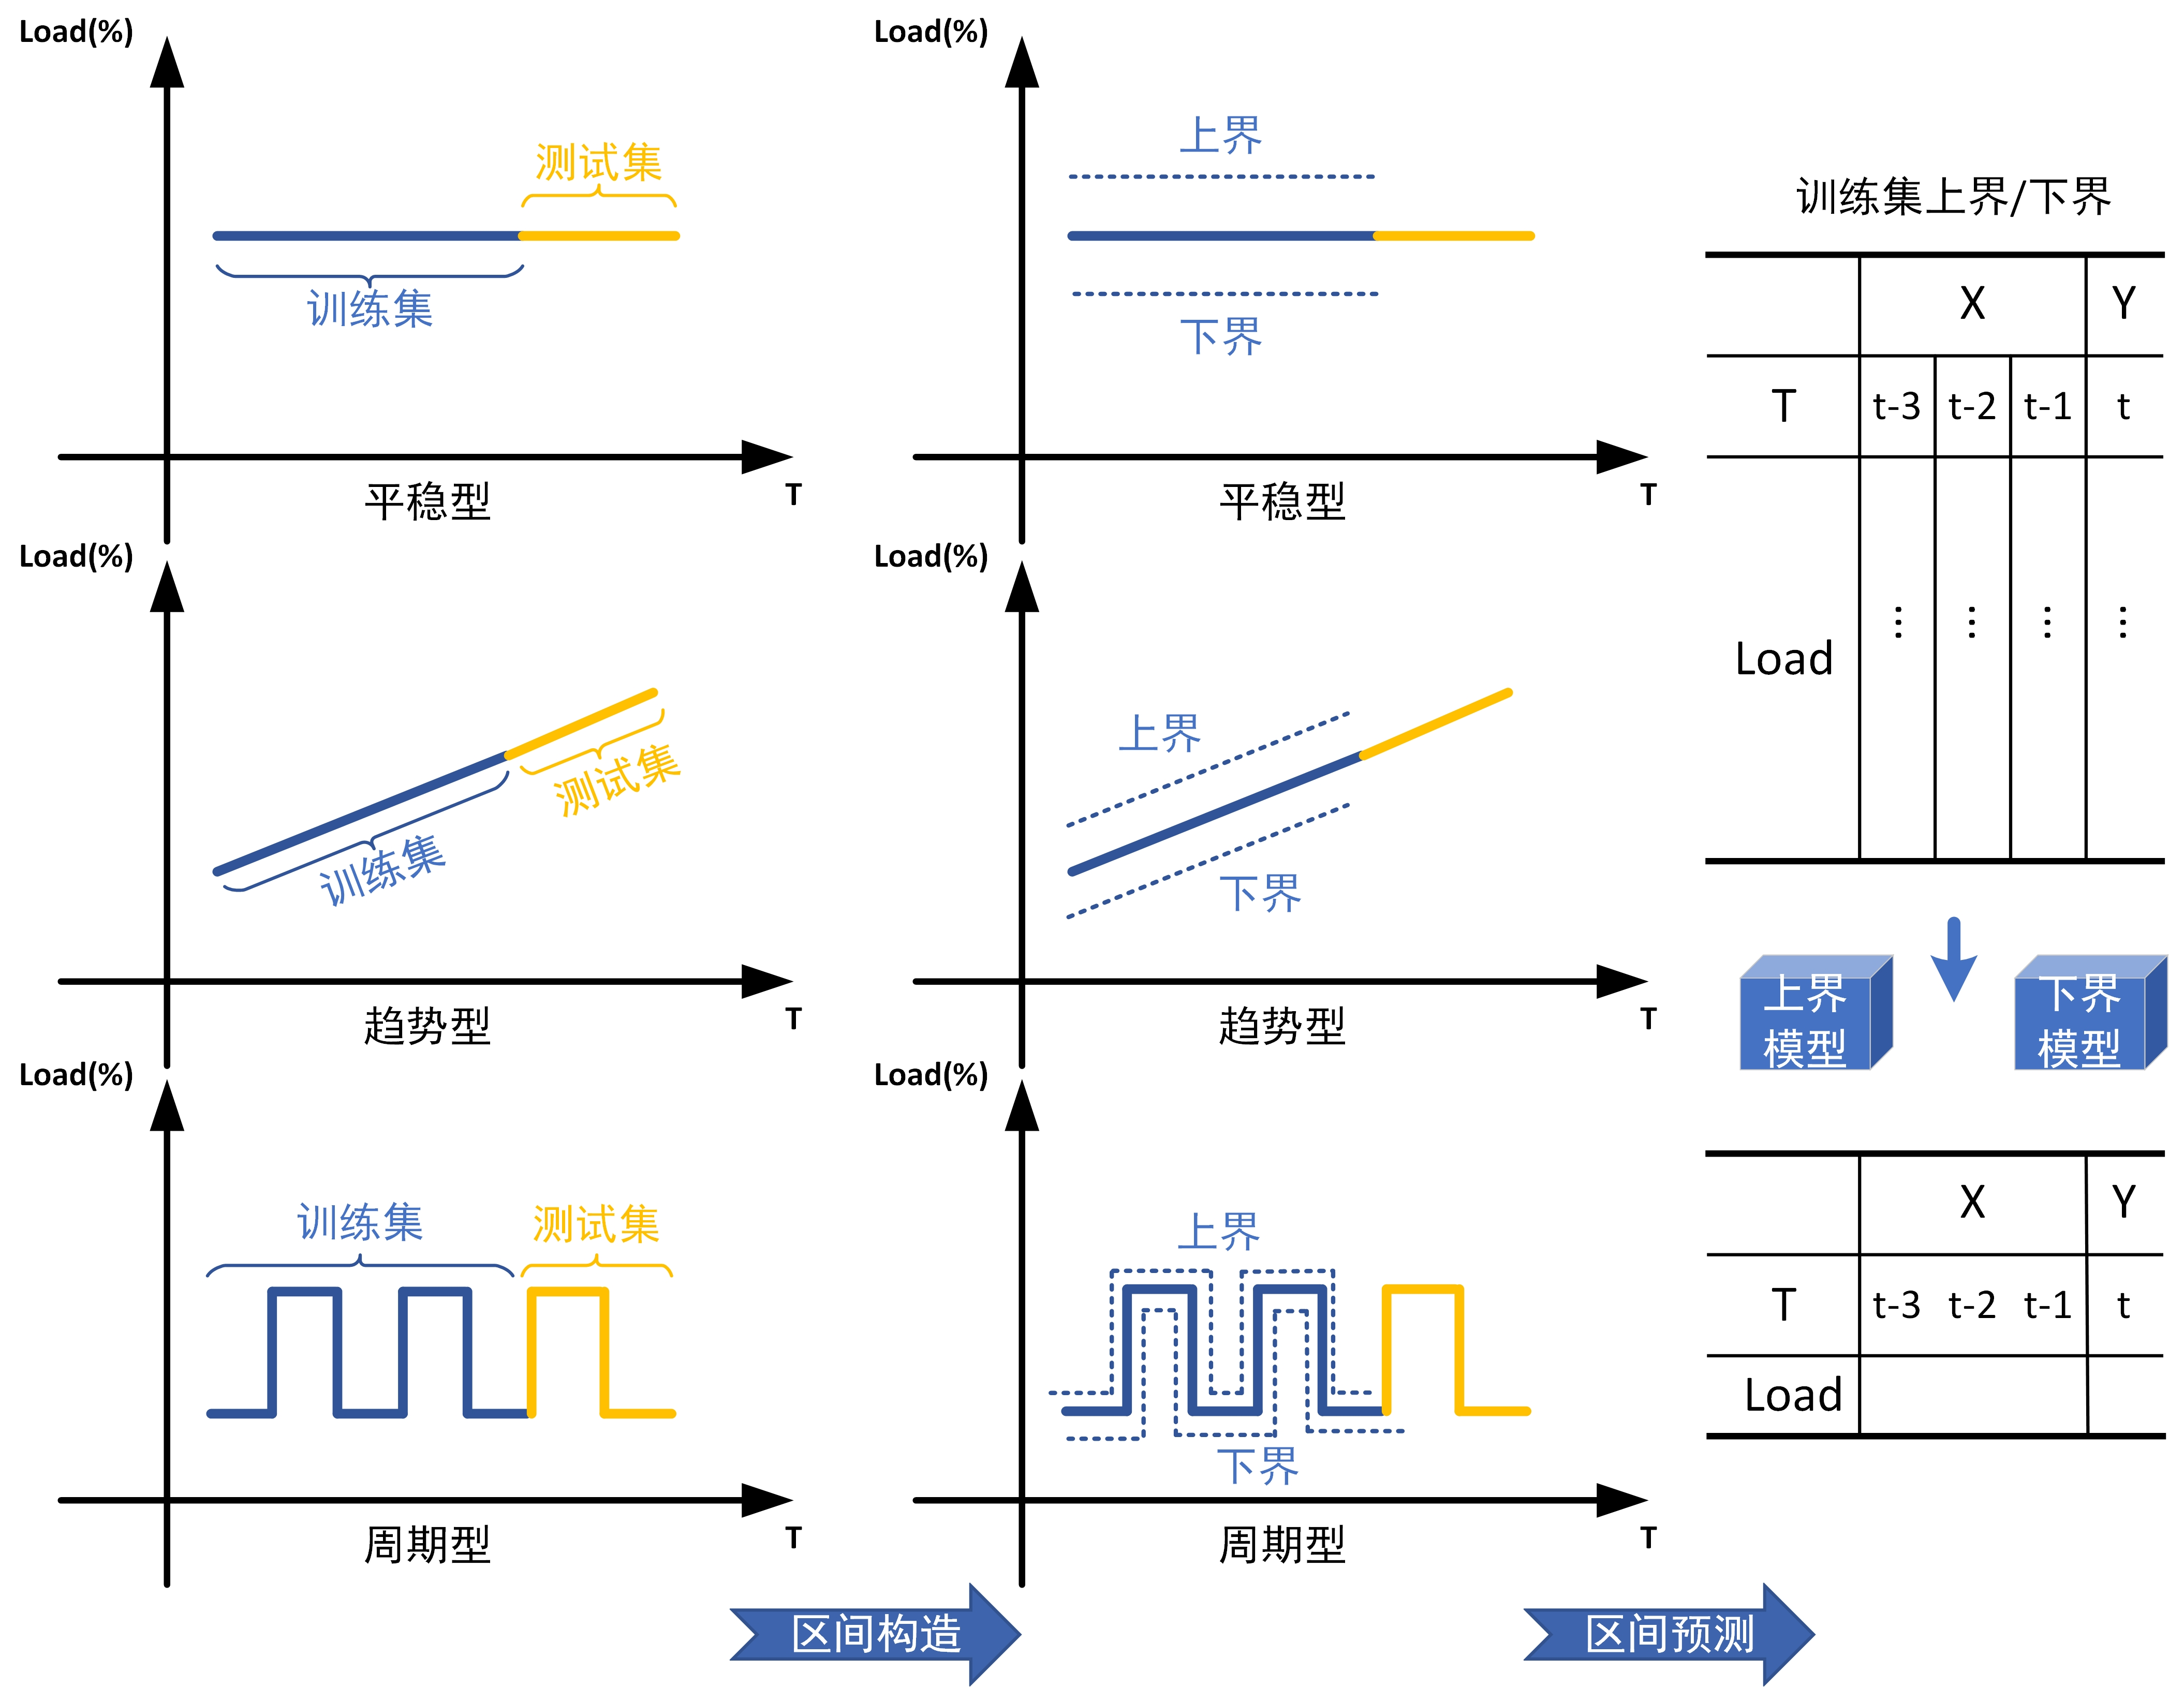
\includegraphics[scale=0.38]{figures/fig7_predict_process.jpg}
\caption{模型预测过程}
\label{fig:fig7}
\end{figure}
\end{column}
\end{columns}
\end{frame}

\subsection{趋势感知}

\begin{frame}
\frametitle{趋势感知}
\framesubtitle{定义}
\begin{itemize}
    \item 容器负载:\textbf{时间段$p$内CPU利用率均值}(\sout{Load Average})
    \begin{equation}
        load = avg(u(p))
    \end{equation}
    \item 负载时序数据
    \begin{equation}
        S=\{(t_1,load_1),(t_2,load_2),\cdots,(t_n,load_n)\}=\{(t_i,load_i)\}|^n_{i=1}
    \end{equation}
    \begin{equation}
        load_i = avg(u(t_i - t_{i-1}))
    \end{equation}
    \begin{itemize}
        \item $t_i - t_{i-1}$ \textbf{增大} $\Rightarrow$ \textbf{$load_i$ 平均特征}
        \item $t_i - t_{i-1}$ \textbf{减小} $\Rightarrow$ \textbf{$load_i$ 瞬时特征}
    \end{itemize}
\end{itemize}
\end{frame}

\begin{frame}
\frametitle{趋势感知}
\framesubtitle{SAC规则}
\begin{itemize}
    \item 频谱特征分析(\textbf{S}pectrum \textbf{A}nalysis)
    和自相关系数(\textbf{A}utocorrelation \textbf{C}oefficient)分析判定规则(SAC规则)
\end{itemize}
\begin{figure}[htb]
\centering
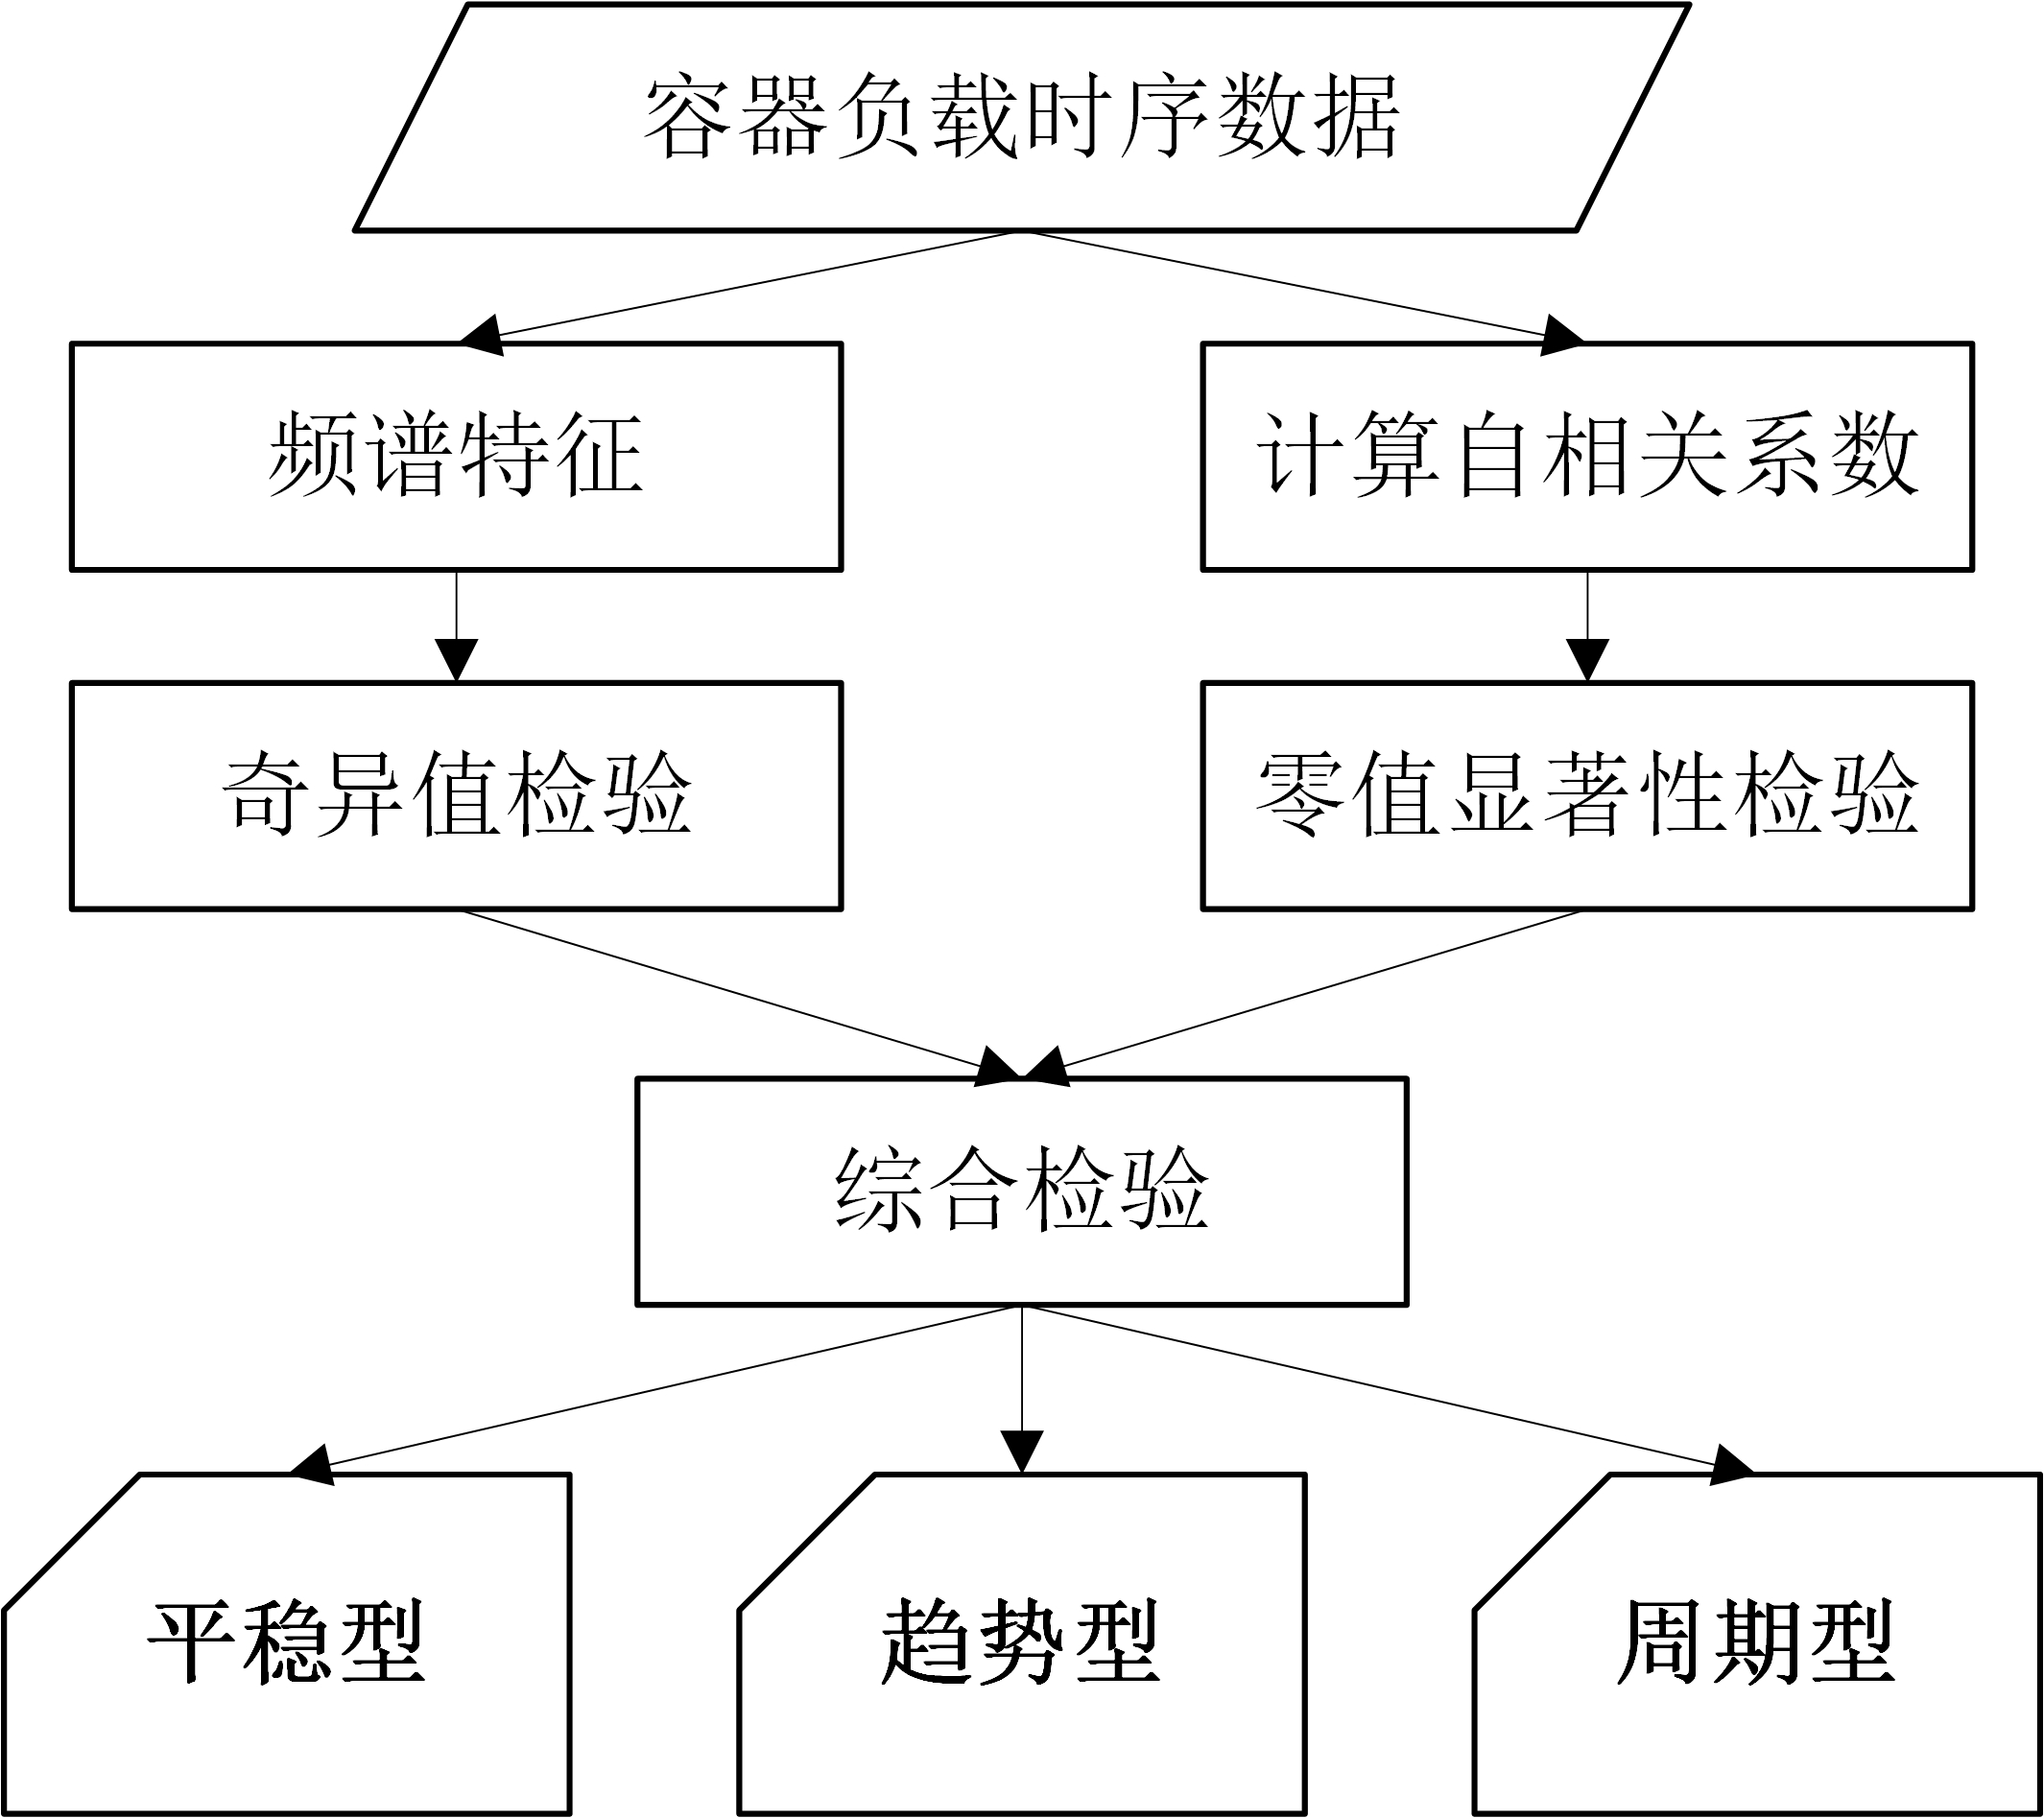
\includegraphics[scale=0.6]{figures/fig8_sac_process.jpg}
\caption{SAC规则实施流程}
\label{fig:fig8}
\end{figure}
\end{frame}

\begin{frame}
\frametitle{趋势感知}
\framesubtitle{SAC - 频谱特征分析}
\begin{enumerate}[1]
    \item 负载数据(\textbf{时域数据}) $\Rightarrow$ 负载信号(\textbf{频域数据})
    \item 频谱特征:负载信号表现出的特征
\end{enumerate}
\begin{block}{负载信号:某一采样频率下,负载在频域上的取值}
    \begin{itemize}
    \item 离散傅立叶变换(DFT)
    \end{itemize}
    \begin{equation}
    \left\{
        \begin{array}{rcl}
        F_{\color{red}{v}} &=& \sum_{j=1}^{n} e^{-i\frac{2\pi}{n}({\color{red}v}-1)(j-1)}load_i,
        {\color{red}v=1,2,\cdots,m} \\
        m &=& \lceil \frac{n}{2} \rceil
        \end{array}
    \right.
    \end{equation}
\end{block}
\begin{block}{频谱特征}
\begin{itemize}
    \item 单个频谱特征
    \begin{equation}
        q_v = \frac{1}{m}\left|F_v \right|^2,v=1,2,\cdots,m
    \end{equation}
    \item 频谱特征序列
    \begin{equation}
        Q = \{q_1,\cdots,q_m\} = \{q_v\}|^m_{v=1}
    \end{equation}
\end{itemize}
\end{block}
\bigskip
\end{frame}

\begin{frame}
\frametitle{趋势感知}
\framesubtitle{SAC - 自相关系数分析}
\begin{enumerate}[1]
    \item 按滞后期$k$,将原时序序列S拆分为两个新序列:$S_{before}$ 和 $S_{after}$
    \begin{itemize}
        \item 前置序列:$s_{before} = \{load_1,load_2,\cdots,load_{n-k}\}=\{load_i\}|^{n-k}_{i=1}$
        \item 前置序列:$s_{before} = \{load_{1+k},load_{2+k},\cdots,load_{n}\}=\{load_i\}|^{n}_{i=1+k}$
    \end{itemize}
    \item 计算滞后期为$k$时的自相关系数:$\bar{S} = \sum_{i=1}^{n} \frac{load_i}{n}$
    \begin{equation}
    \begin{aligned}
        \rho_k & =  \frac{\gamma(i,i+k)}{Var(S)} \\
               & = \frac{\sum_{i=1}^{n-k} (load_i - \bar{S})(load_{i+k} - \bar{S})}{\sum_{i=1}^{n} (load_i - \bar{S})^2}
    \end{aligned}
    \end{equation}
    \item 获得自相关系数序列:$k=1,2,\cdots,m$, $m = \lceil \frac{n}{3} \rceil$
    \begin{equation}
        P = \{\rho_1,\rho_2,\cdots,\rho_m\} = \{\rho_k\}|^m_{k=1}
    \end{equation}
\end{enumerate}
\bigskip
\end{frame}

\begin{frame}
\frametitle{趋势感知}
\framesubtitle{SAC - 判定}
    \begin{itemize}
        \item 周期性判定:奇异值检验
        \begin{enumerate}[1]
            \item 计算频谱特征序列$Q=\{q_v\}|^m_{v=1}$的差分序列$H = \{h_v\}|^{\lceil \frac{m}{2} \rceil}_{v=2}$
            \begin{equation}
                h_v = \left|(q_v - q_{v+1}) + (q_v - q_{v-1})\right|,v=2,3,\cdots,\lceil \frac{m}{2} \rceil
            \end{equation}
            \item 计算序列$H$的均值$\mu_H$和标准差$\sigma_H$
            \item $3\sigma$标准:序列$Q$中存在$q_v$使对应的差分项$h_v$满足如下条件
            \begin{equation}
                h_v - \mu_H > 3\sigma_H
                \label{eq:3sigma}
            \end{equation}
        \end{enumerate}
        \item 平稳性判定:显著性检验
        \begin{enumerate}[1]
            \item $t$-检验 $\Rightarrow$ H0:序列平稳,H1:序列不平稳,显著性水平:$\alpha=0.05$
            \item 计算自相关系数序列$P$总体与零值相关概率$P_\rho$
            \item 检验标准
            \begin{itemize}
                \item $P_\rho \geq \alpha$ $\Rightarrow$ 接受H0假设
                \item $P_\rho < \alpha$ $\Rightarrow$ 接受H1假设
            \end{itemize}
        \end{enumerate}
    \end{itemize}
\end{frame}

\begin{frame}
\frametitle{趋势感知}
\framesubtitle{SAC - 判定}
\begin{block}{负载类型定义}
    \begin{itemize}
        \item 平稳型负载:不存在$q_v$,使$h_v$满足公式\ref{eq:3sigma},且$P_\rho \geq \alpha$
        \item 趋势型负载:不存在$q_v$,使$h_v$满足公式\ref{eq:3sigma},且$P_\rho < \alpha$
        \item 周期型负载:存在$q_v$,使$h_v$满足公式\ref{eq:3sigma}
    \end{itemize}
\end{block}
\end{frame}

\subsection{区间构造}

\begin{frame}
\frametitle{区间构造}
\end{frame}


\subsection{区间预测}

\begin{frame}
\frametitle{区间预测}
\end{frame}


\subsection{实验结果与分析}

\begin{frame}
\frametitle{实验结果与分析}
\end{frame}